%=====================================================================
\section{Experimental record and results}\label{sec:results}
%=====================================================================
All runs start from a straight chain with a $10^{-8}$ sine jitter. Throughput is about $1.0$--$1.4\times10^5$ steps/s per core with the Verlet list
(brute force: $4.9\times10^4$).

\subsection{Session 1: integrity smoke runs}
\textbf{Requested smoke} (\code{polymer}, $\Pe=200$, 4000 steps $=0.2$ time units, plus a $\Pe=0$ reference):
\begin{itemize}
\item The unwrapped COM moves from $(0,6.3\times10^{-9})$ to $(-0.0160,0.1259)$, $|\Delta|=0.127$, and is never reset. This displacement is thermal: $v_0t\approx0.004$ against $\sqrt{4D_tt}\approx0.09$.
\item $\max|\spn|=0.137$ and the median $|\spn|=0.054$.
\item The railway touch is physically impossible in this window: a bead moves $0.02r_0$ per time unit, the $i=1$ transit needs about 50 time units, and the maximum lag was 0.1.
\end{itemize}
\textbf{Supplementary integrity run} (\code{weak_spiral}, $\Pe=1000$, $2\times10^6$ steps $=100$ time units, sampled every 1000 steps, with a passive reference):
\begin{center}\small
\begin{tabular}{ccccc}\toprule $i$ & predicted transit $ir_0/v$ & lag of min.\ ratio & $\min\ \mathrm{MSD}_{j+i}/\mathrm{MSD}_\mathrm{passive}$ & note\\ \midrule
1 & 10 & 14.8 & 0.982 & \\ 2 & 20 & 21.9 & 0.878 & \\ 4 & 40 & 40.2 & 0.69 & near window edge\\ 8 & 80 & 42 & 2.87 & transit not reached\\ \bottomrule\end{tabular}
\end{center}
The minima sit near the predicted transits and touch the passive curve: railway motion, qualitatively as in Fig.~6.
Ratios below 1 come from one seed with few independent origins at long lag, and are not significant. In this run the unit-slope rule returned
$D=1.27\times10^{-4}$ on $t\in[1.15,1.75]$. That is a short-lag crossover, not the diffusive regime ($1/D_{r,a}\approx200$ is longer than the window),
which shows the rule is mechanical and must be inspected.

\subsection{Session 2: visual integrity runs ($2\times10^6$ steps $=100$ time units $=3.96\times10^{-4}\tau$ each)}
\begin{figure}[H]\centering
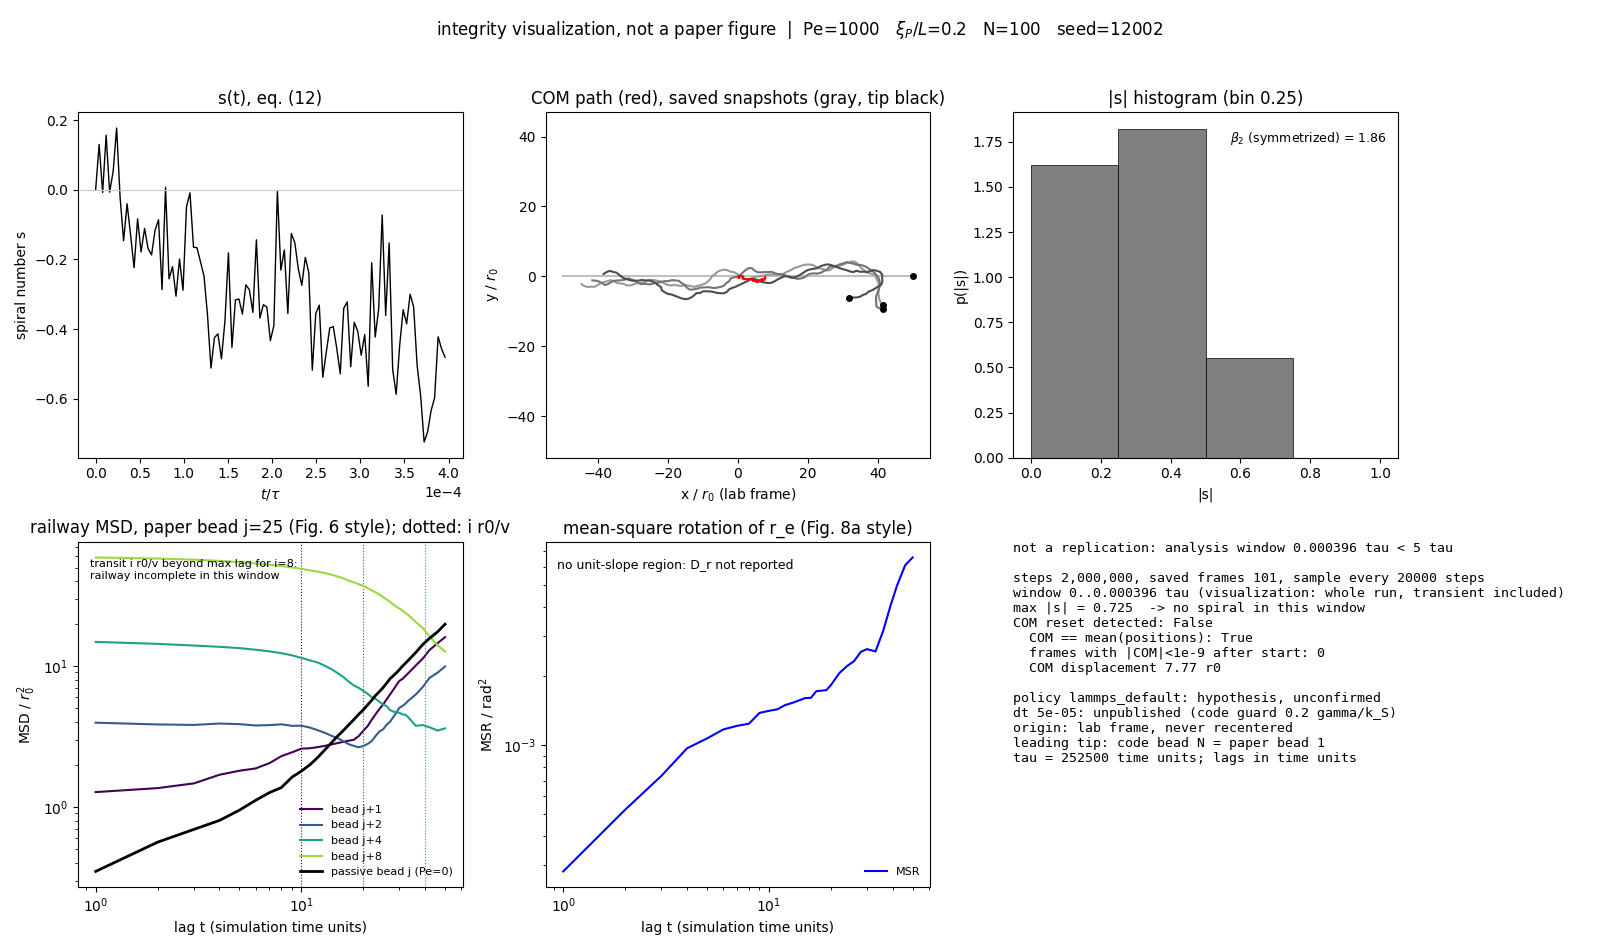
\includegraphics[width=\linewidth]{viz_weak.png}\\[0.5em]
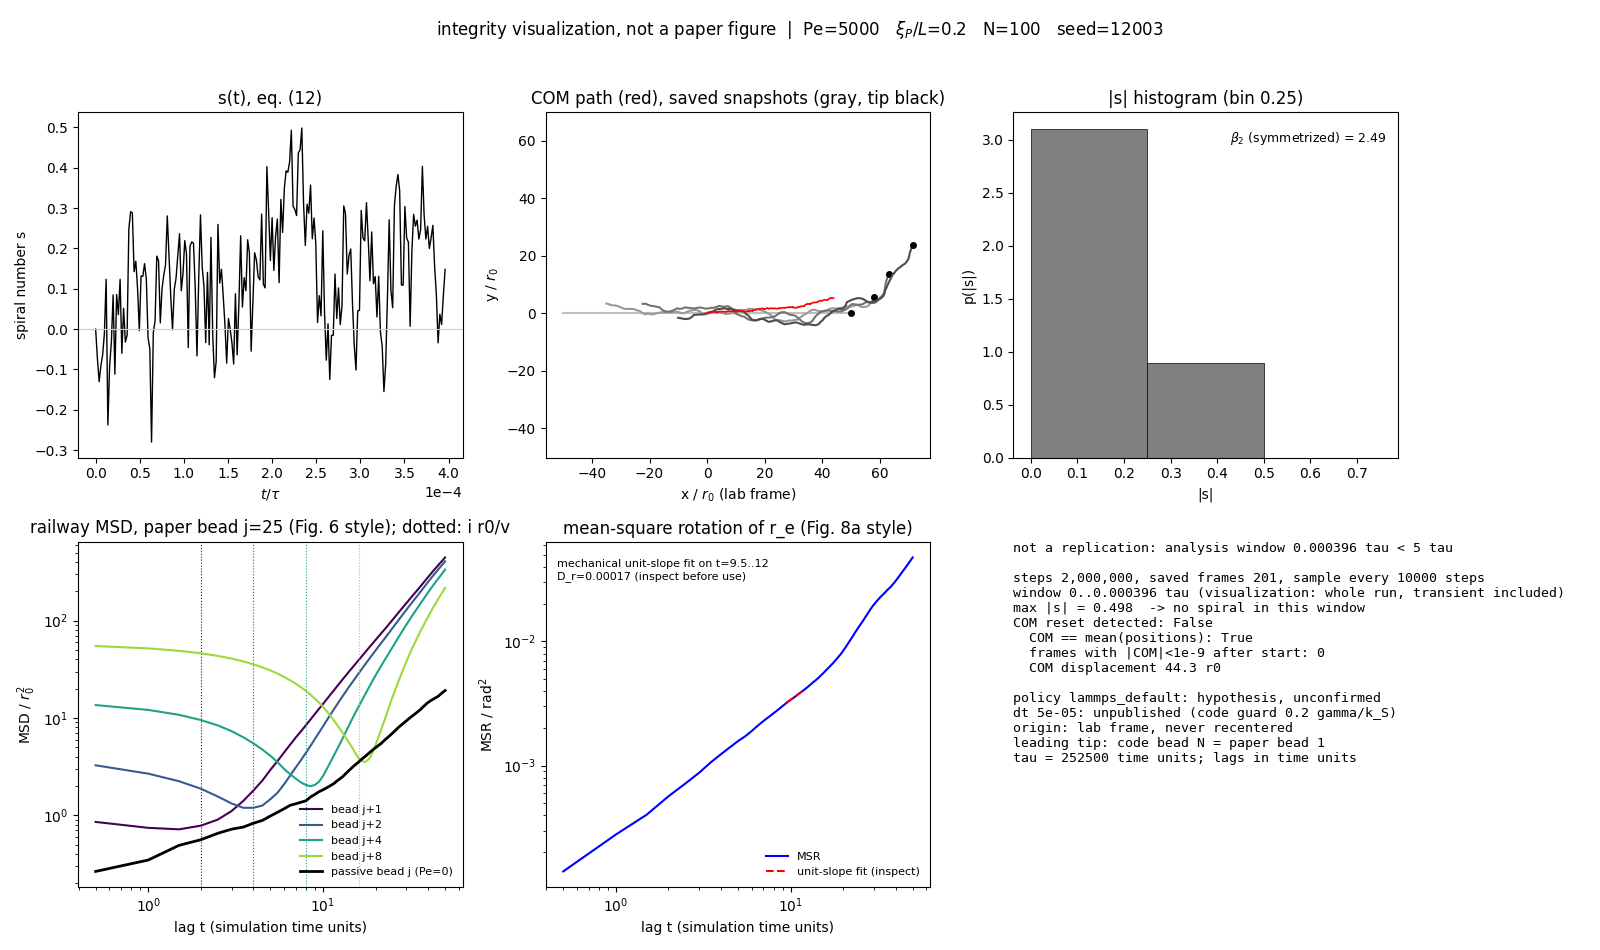
\includegraphics[width=\linewidth]{viz_strong.png}
\caption{Integrity panels (session 2): weak-spiral (top) and strong-spiral (bottom) presets over 100 time units. Panels: $\spn(t)$, COM path with snapshots,
$|\spn|$ histogram, railway MSD against the passive reference, MSR. Not paper figures.}
\end{figure}
\begin{center}\small
\begin{tabular}{lcccc}\toprule run & frames (film) & $\max|\spn|$ & COM displacement & COM reset? \\ \midrule
polymer $\Pe=200$ & 101 (101) & 0.427 & 2.58 & no \\ weak $\Pe=1000$ & 101 (101) & 0.725 & 7.77 & no \\
strong $\Pe=5000$ & 201 (101, stride 2) & 0.498 & 44.3 & no \\ \bottomrule\end{tabular}
\end{center}
No spiral formed in any of these windows; 100 time units is half a contour at $\Pe=5000$, so none was expected. The unit-slope rule again fitted early
crossovers: $9.6\times10^{-5}$ for the polymer run and $1.7\times10^{-4}$ for the strong run. Neither is a result.

\subsection{Session 3: the first formation gate}
Ten contours at $\Pe=5000$ ($4.04\times10^7$ steps, 401 frames at 0.025 contour, about 5--6 min each):
\code{lammps_default}/12003 had $\max|\spn|=1.68$ and failed; \code{paper_all_pairs}/12013 held $\spn\approx-4.1$ from 4.8 to 8.6 contours
(153 frames, 3.80 contours, $\max|\spn|=4.44$) and passed. Both COM checks were clean.
A $5\tau$ job was then launched with \code{paper_all_pairs} and the preset seed \emph{12003}, at the then-default cadence of $0.01\tau$.
This was the wrong job, as described next.

\subsection{Session 4: the wrong job, and the unconfounded gate}
\begin{warnbox}[title=Correction]
The job above used a seed (12003) that had been gated only under the other policy, where it failed. Its cadence ($0.01\tau=12.5$ contours) was also coarser than the only measured plateau (3.8 contours).
It was stopped at step $78\,780\,000$ (19.5 contours; last checkpoint $50\,500\,000$), was not resumed, and its folder is marked \code{STOPPED}.
\end{warnbox}
The gate was then repeated with the policy--seed pairs crossed:
\begin{figure}[H]\centering
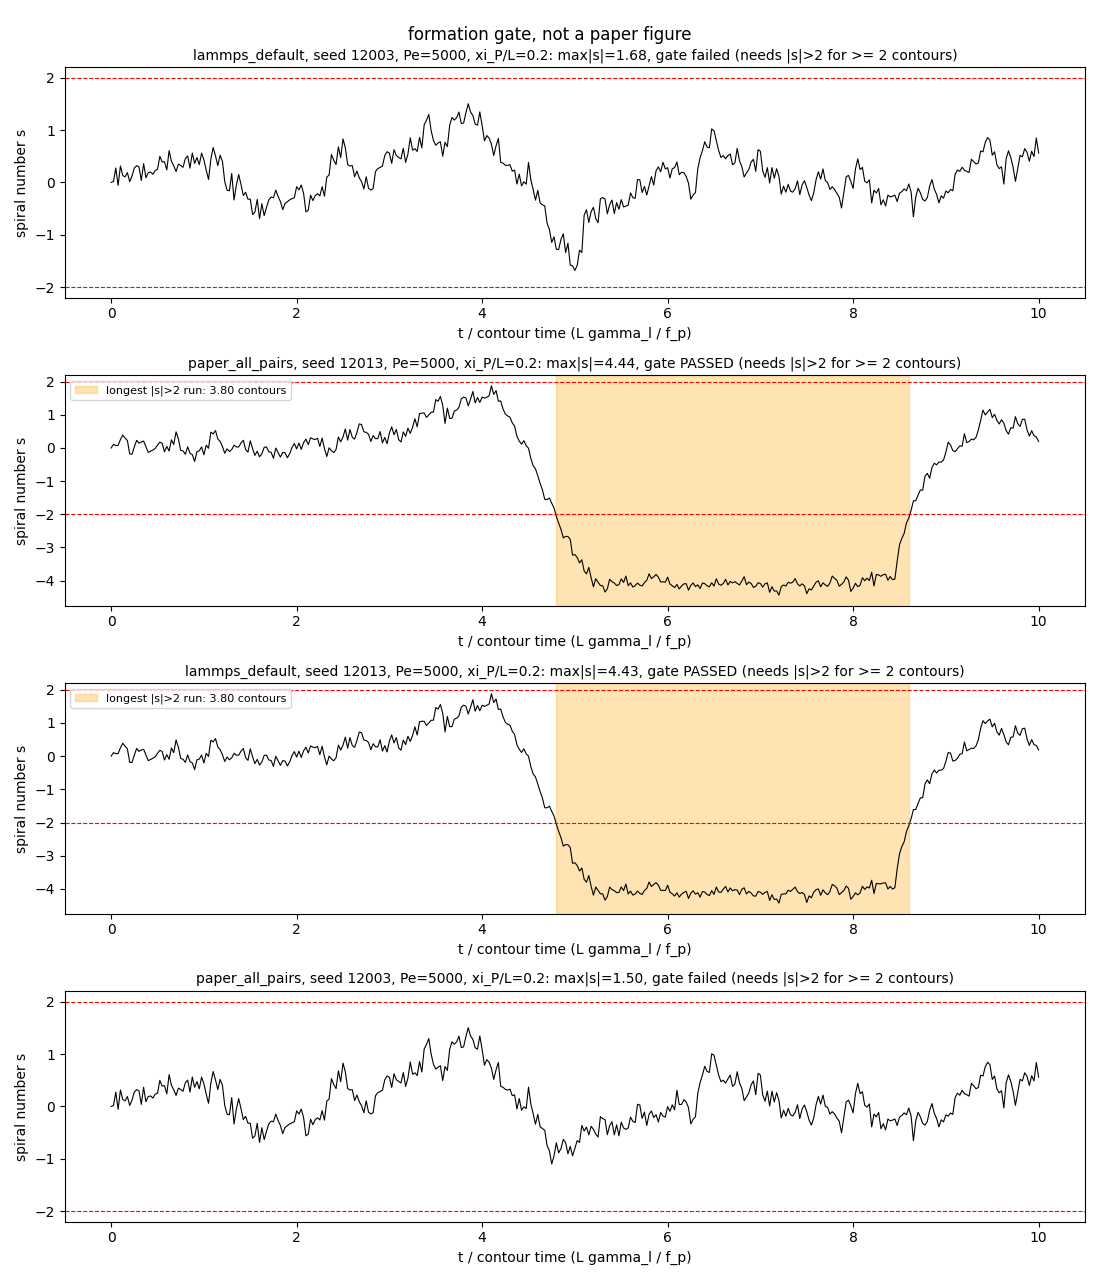
\includegraphics[width=0.84\linewidth]{gate4_s_t.png}
\caption{Unconfounded formation gate (10 contours each). Shaded: the longest $|\spn|>2$ run. Formation follows the seed, not the policy.}
\label{fig:gate4}
\end{figure}
\begin{center}\small
\begin{tabular}{llcccc}\toprule policy & seed & $\max|\spn|$ & longest $|\spn|>2$ run & COM check & gate\\ \midrule
\code{lammps_default} & 12003 & 1.68 & none & clean & fail\\
\code{paper_all_pairs} & 12013 & 4.44 & 3.80 contours (4.8--8.6) & clean & \textbf{pass}\\
\code{lammps_default} & 12013 & 4.43 & 3.80 contours (4.8--8.6) & clean & \textbf{pass}\\
\code{paper_all_pairs} & 12003 & 1.50 & none & clean & fail\\ \bottomrule\end{tabular}
\end{center}
\textbf{Interpretation.} Under a fixed seed, both policies consume the same noise stream; they differ only in the WCA forces between beads at most three bonds apart.
Formation is caused by tip--body contact at large separation, so the two trajectories stay close, and the gate cannot discriminate the policies.
Two seeds do not estimate a formation rate.

\begin{figure}[H]\centering
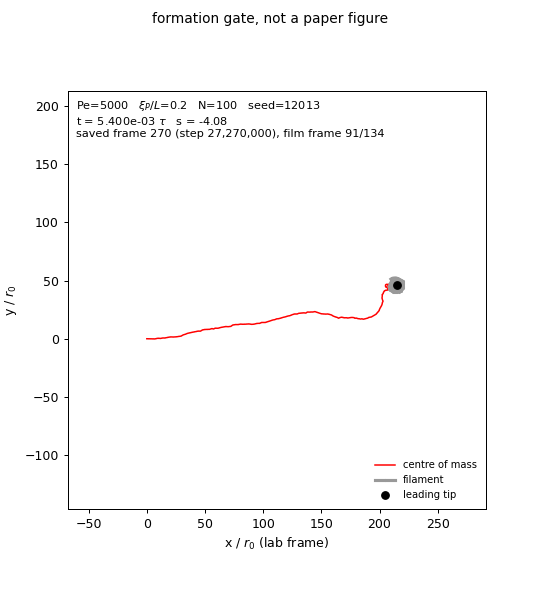
\includegraphics[width=0.42\linewidth]{frame_gate_lab.png}\hfill
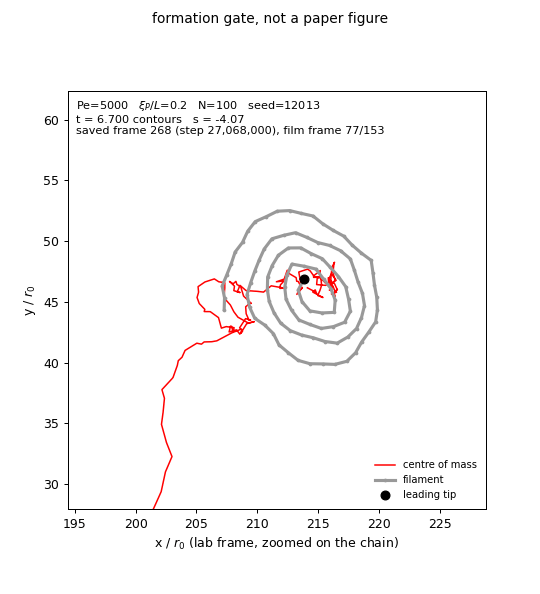
\includegraphics[width=0.42\linewidth]{frame_gate_plateau.png}
\caption{Seed 12013 gate film frames. Left: lab-frame box over the whole 250-$r_0$ trail ($\spn=-4.08$, $t=5.4\times10^{-3}\tau$). Right: zoom on the wound chain
(about four turns, leading tip black at the centre, COM wandering diffusively).}
\end{figure}

\subsection{Session 5--6: the $5\tau$ trajectory}
\begin{itemize}
\item \textbf{Configuration.} \code{strong_spiral}, \code{paper_all_pairs}, seed 12013; $25\,250\,000\,000$ steps; one frame every $1\,010\,000$ steps (0.25 contour), 25\,001 frames;
a checkpoint at every frame (about every 9\,s). Because the integrator is deterministic, the first 10 contours repeat the passing gate run exactly.
\item \textbf{Segment 1.} Started 2026-10-02 01:38:22 (+05:30). Stopped 03:38:09 at step $862\,540\,000$ ($0.171\tau$, 213.5 contours), with empty stderr and no reboot or sleep.
Fourteen seconds later the Windows log shows a service installation and the ``Claude'' service set to disabled.
The likely cause is an application update terminating its process tree; the timing is suggestive but not proof.
A read-only check showed the segment intact: 855 frames ending exactly at the checkpoint step, COM $\equiv$ mean of the positions, \code{complete=False}.
\item \textbf{Segment 2.} Resumed by the user (double-clicking \code{resume1.cmd}) on 2026-10-03 00:50:29 and completed 2026-10-05 06:03:49.
Segment wall time $191\,598$\,s (53.2\,h) for $2.4387\times10^{10}$ steps, i.e.\ $1.27\times10^5$ steps/s. The run reports a cumulative \code{wall_seconds} of $198\,785$\,s, because the checkpoint carries segment~1's time forward. The physics fingerprint is unchanged.
\item \textbf{Stitch.} 25\,001 frames from step 0 to $2.525\times10^{10}$, \code{complete=True}, bitwise-equal shared frame.
\end{itemize}

\begin{figure}[H]\centering
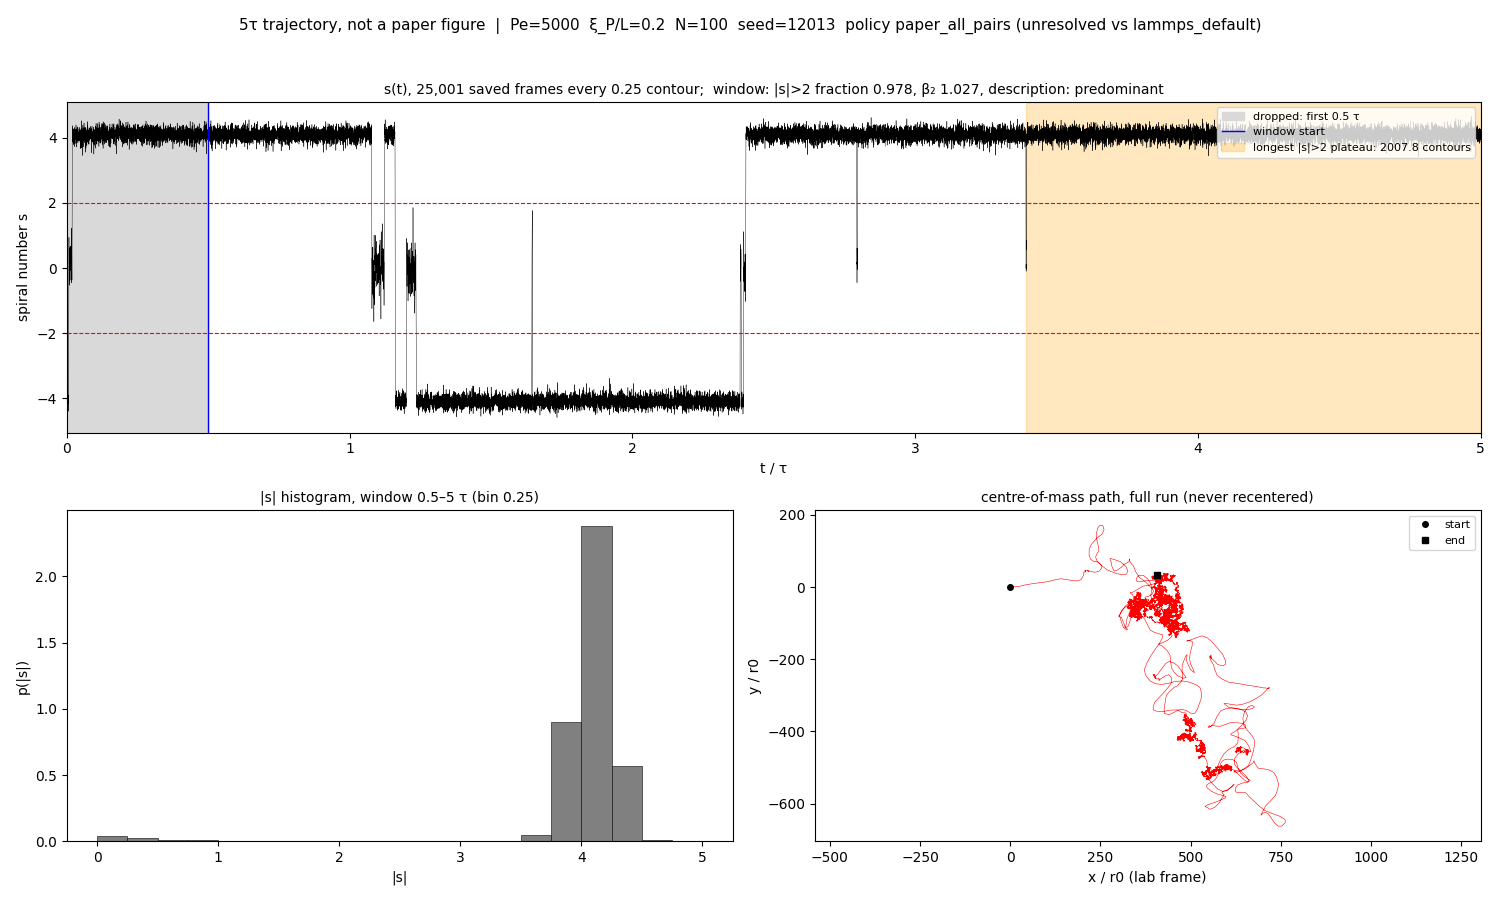
\includegraphics[width=\linewidth]{result_panel.png}
\caption{The $5\tau$ trajectory (seed 12013, $\Pe=5000$, $\xiP/L=0.2$). Top: $\spn(t)$, with the dropped first $0.5\tau$ shaded and the longest plateau highlighted.
Bottom left: window $|\spn|$ histogram. Bottom right: lab-frame COM path. Not a paper figure.}
\label{fig:result}
\end{figure}

\begin{table}[H]\centering
\caption{Verdict on the window $0.5$--$5.0\tau$ (22\,501 samples).}\label{tab:verdict}
\begin{tabular}{lr}\toprule
Description(s) & \textbf{predominant} \\
Fraction of samples with $|\spn|>2$ & 0.978 \\
Symmetrized $\beta_2$ & 1.027 \\
Longest plateau & $\geq$ 2007.75 contours ($\approx1.61\tau$; censored at run end) \\
COM MSD log--log slope & 1.001 \\
Unit-slope MSR region after $0.5\tau$ & none, so $D_r$ = null \\
$|\spn|$ in $[3.5,4.75)$ / $|\spn|<1$ & 97.7\% / 1.95\% (mode bin $[4.0,4.25)$) \\
Net COM displacement over $5\tau$ & 408.5 $r_0$ \\ \bottomrule
\end{tabular}
\end{table}

\begin{figure}[H]\centering
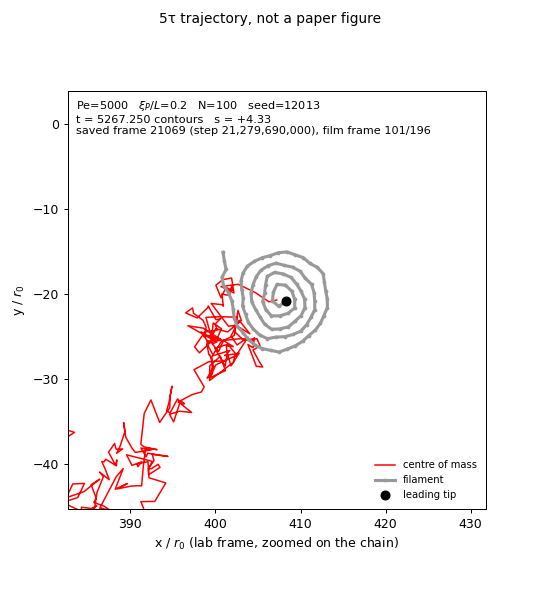
\includegraphics[width=0.45\linewidth]{frame_result_plateau.png}
\caption{Frame 101 of the 196-frame film of the longest plateau. The box follows the COM ($\pm24.6r_0$); the red trail starts at the plateau. $\spn=+4.33$ at $t=5267$ contours.}
\end{figure}

%=====================================================================
\section{Analysis and discussion}\label{sec:analysis}
%=====================================================================
\subsection{What the $5\tau$ trajectory shows}
\begin{itemize}
\item \textbf{Dynamics of $\spn$.}
\begin{itemize}
\item A spiral forms within the first few contours.
\item $\spn\approx+4$ holds until about $1.08\tau$; there are brief break-ups between $1.08$ and $1.24\tau$.
\item $\spn\approx-4$ holds from $1.24$ to about $2.4\tau$, then $\spn\approx+4$ to the end.
\item Single-frame dips occur near $2.8\tau$ and $3.39\tau$.
\item Spirals break up and re-form with either handedness. In the language of Fig.~4e this seed behaves like a light-red (break-up) strong-spiral point, not a dark-red (never breaks) one.
\end{itemize}
\item \textbf{Distribution.} The histogram has a minute low-$|\spn|$ peak (elongated state) and a dominant peak at $|\spn|\approx4$. Qualitatively this is the Fig.~4c description for $\Pe=5000$.
The low symmetrized $\beta_2$ ($\approx1$, the value for a two-point distribution at $\pm a$) is what the paper describes for spiral-dominated runs.
\item \textbf{Translation.} The COM path shows dense diffusive clusters while wound, linked by long directed excursions while elongated, the ``separated clusters'' of the Fig.~2 caption.
The long-lag COM MSD slope of 1.00 matches the paper's statement that translation in the spiral state is almost purely diffusive.
\item \textbf{Rotation.} No unit-slope MSR region appears. The paper likewise reports that the long-time MSR $\propto t$ regime ``could not be detected'' for runs with spontaneous break-up.
\end{itemize}

\subsection{Where this sits against the paper's claims}
\begin{center}\small
\begin{tabular}{p{0.42\linewidth}p{0.48\linewidth}}\toprule Paper's claim & Status here\\ \midrule
Tip collision winds the chain into a spiral at high $\Pe$, low $\xiP/L$ (Fig.~3a) & Observed (seed 12013), tip at the centre\\
Spiral state dominates at $\Pe=5000,\xiP/L=0.2$ (Fig.~2c, 4b--c) & Predominant on one seed over $4.5\tau$\\
$\beta_2\ll3$ when spirals dominate (Fig.~4d) & $\beta_2=1.03$ (one seed; values not compared numerically)\\
No spirals at $\Pe=200$ (Fig.~2a) & Consistent in a 100-time-unit run only\\
Railway motion; MSD minima touch passive (Fig.~6) & Seen qualitatively in a 100-time-unit run at $\Pe=1000,\xiP/L=0.2$\\
Formation depends on $(\Pe,\xiP/L)$ & Over 10 contours it depended on seed: 12003 did not wind\\
\bottomrule\end{tabular}
\end{center}

\subsection{Caveats that bound every statement}
\begin{enumerate}
\item \textbf{One seed, one point.} The verdict describes one trajectory. Seed-to-seed variability is unknown.
\item \textbf{Censoring.} The longest plateau ends with the run, so 2007.75 contours is a lower bound on its lifetime.
\item \textbf{Cadence.} At 0.25 contour per frame (50.5 time units), events shorter than a frame are invisible. Single-frame dips split plateaus under the consecutive-frame rule.
Fig.~6 needs about 2 time units per frame at $\Pe=5000$ and cannot be computed from this file.
\item \textbf{Policy unresolved.} The same seed gives the same formation under both policies; break-up statistics might differ, but that is untested.
\item \textbf{Timestep unpublished.} $\Delta t$ is a conservative guard. A different ESI value could shift break-up rates, which depend on tip curvature.
\item \textbf{Quantitative comparison absent.} The paper's figure values were not digitized, so ``consistent'' means qualitatively consistent.
\end{enumerate}

%=====================================================================
\section{Verification and audit status}\label{sec:tests}
%=====================================================================
\subsection{Test inventory (64 tests, all passing)}
Every new test has one assertion, and none merely checks that a number is finite.
\begin{longtable}{p{0.26\linewidth}p{0.06\linewidth}p{0.6\linewidth}}
\toprule file & n & what it establishes \\ \midrule\endhead
\code{test_forces.py} & 3 & finite-difference gradient of $U$; Newton's third law and net propulsion $f_p(\vect r_N-\vect r_0)$; policies differ\\
\code{test_engine_io.py} & 5 & chunk invariance (brute and Verlet); checkpoint round trip and fingerprint refusal; HDF5 sampling; overwrite refusal\\
\code{test_observables.py} & 6 & spiral number of an Archimedean spiral; Gaussian kurtosis; streaming moments; Kratky--Porod value; ballistic MSD slope; static $S(q,t)$\\
\code{test_paper.py}, \code{test_parameters.py} & 5 & Fig.~2 presets; $\tau=252\,500$; $5\tau$ step count; $\Delta t$ guard; $\kappa=20$, $f_p=0.5$, $\Flex=25\,000$\\
\code{test_origin.py} & 8 & COM not reset at the old boundary; stored positions equal an independent un-recentered integration; COM $\equiv$ mean of positions; recenter refused without offset; offset restores lab frame; resume equals uninterrupted (positions, angle); chunk size irrelevant\\
\code{test_figures.py} & 14 & unwrapping; railway minimum at transit; $D_r$ fit and its refusal; $\tau_S$ of an exponential; $S(q,t)$ translation phase; $\beta_2=1$ for constant $|\spn|$; histogram bins; leading-tip map; policy defaults agree; lags in time units; window; schema-2 refusal; plateau rule\\
\code{test_visualize.py} & 6 & refusal without \code{origin_convention}; frame cap; GIF frames are saved frames; reset detector; plateau films (fixed and following)\\
\code{test_reproduce_cli.py} & 10 & default 0.25 contour; $\tau$ and step units; resume equals uninterrupted; earlier segment kept; stitch equals uninterrupted; stitch refuses gap, overlap and a second origin; \code{--seed}\\
\code{test_verdict.py} & 7 & one synthetic series per description; $0.008\tau$ file refused; missing origin refused; altered COM refused; window starts at $0.5\tau$\\ \bottomrule
\end{longtable}

\subsection{Verified and unverified}
\begin{okbox}[title=Verified]
Force law against both sources; energy gradient; propulsion total; bitwise determinism under chunking, resume and stitching; lab-frame single origin across all stored frames and segments;
index map; every observable against an analytic or synthetic case; COM integrity of every production and gate file used.
\end{okbox}
\begin{warnbox}[title=Unverified or open]
\begin{itemize}
\item \textbf{Inputs.} ESI timestep; the original \code{special_bonds}; which policy the paper used.
\item \textbf{Generality.} Seed-to-seed reproducibility of formation and dominance.
\item \textbf{Comparison.} Quantitative agreement with any figure.
\item \textbf{Analysis.} Figs.~5, 8, 9, 10 analyses on the $5\tau$ file (the code exists; not yet run on it).
\end{itemize}
\end{warnbox}

\subsection{Known weaknesses in the tree}
\begin{itemize}
\item \code{paper.audit()} still reports \code{paper_faithful = (policy == 'lammps_default')}. It is a string comparison, not evidence; \code{paper.py} was outside the edit scope.
\item The $D_r$ unit-slope rule can lock onto a crossover; inspect the MSR before trusting a value.
\item GIF delays are quantised to 10\,ms, so the requested 12\,fps plays at 12.5\,fps (80\,ms per frame).
\item \code{analyze()} reads one file; multi-segment data must be stitched first.
\item An HDF5 file being written must not be opened by another process. HDF5 is not journaled, so a crash during a metadata write could corrupt a segment. The flush-before-checkpoint order limits the exposure.
\end{itemize}

\subsection{Incident log (errors made and how they were handled)}
\begin{enumerate}
\item \textbf{Test expectation error (session 1).} The first $S(q,t)$ translation test ignored the $|\rho_0(\hat q)|^2$ weighting. The test was corrected; the kernel was not changed.
\item \textbf{No-op typo (session 1).} \code{msr/2*2} in a fit call was removed before any run.
\item \textbf{Misleading diagnostic (session 1).} The smoke script first located the railway minimum with \code{argmin} of the MSD, which picks the short-lag $r_0^2$ plateau. It was replaced by the minimum of $\mathrm{MSD}_{j+i}/\mathrm{MSD}_\mathrm{passive}$.
\item \textbf{Wrong production job (session 3).} The job used seed 12003 at $0.01\tau$ cadence. It was stopped on request, not resumed, and superseded by session~4.
\item \textbf{Path slip (session 5).} A Unix-style path passed into Windows Python created \texttt{C:\textbackslash c\textbackslash\ldots}. It held only two scratch files, was verified, and was removed.
\item \textbf{Job killed by an application update (session 5--6).} The launch was a child of the app. The user restarted it from their own session; that is the recommended launch mode.
\item \textbf{Permissions.} The auto-mode classifier blocked registering a scheduled task, a detached launch from the agent, and the agent editing its own settings. These are by design.
\end{enumerate}

%=====================================================================
\section{Codebase reference}\label{sec:code}
%=====================================================================
\subsection{Layout}
\begin{longtable}{p{0.31\linewidth}p{0.06\linewidth}p{0.56\linewidth}}
\toprule module & lines & responsibility \\ \midrule\endhead
\code{parameters.py} & 64 & frozen \code{Parameters}: dimensionless inputs mapped to $\kappa,f_p,k_S,\gl,\tau,t_c$; \code{dt} guard; policy codes; SHA-256 \code{fingerprint()} of the canonical physics\\
\code{paper.py} & 10 & \code{FIG2} presets; \code{make(regime,policy)}; \code{audit()} (cost estimate)\\
\code{rng.py} & 22 & SplitMix64; 53-bit uniform; keyed Box--Muller \code{normal_pair(seed,step,bead)}\\
\code{forces.py} & 40 & all-pairs reference kernel with energies (used by tests)\\
\code{engine.py} & 95 & \code{straight()}; brute and Verlet integrators; opt-in recentering with offset; \code{benchmark()}\\
\code{simulator.py} & 51 & \code{run()}: sampling, angle unwrapping grid, flush, checkpoint, angle sidecar, resume\\
\code{io.py} & 51 & \code{strict_json}; \code{H5Trajectory} (schema 3, provenance attributes)\\
\code{checkpoint.py} & 18 & atomic \code{npz} save; load with schema and fingerprint checks\\
\code{observables.py} & 85 & every observable in Section~\ref{sec:observables}\\
\code{moments.py} & 10 & streaming fourth moment (symmetrized)\\
\code{analysis.py} & 87 & \code{analyze()}: the second program, a window-explicit Figs.~4--10 input set\\
\code{stitch.py} & 61 & \code{read_segments}, \code{write_stitched}\\
\code{visualize.py} & 141 & films, panels, \code{plateau_film}, COM reset check\\
\code{cli.py} & 61 & command-line interface (Section~\ref{sec:ops})\\
\code{hardware.py}, \code{taichi_backend.py} & 22 & probes only; Vulkan is never used in production\\ \midrule
\code{tests/smoke_integrity.py} & 36 & smoke driver: active run, passive run, analysis\\
\code{tests/formation_gate.py} & 39 & gate evaluator and multi-curve $\spn(t)$ plot\\
\code{tests/verdict.py} & 75 & verdict program\\
\code{tests/result_figures.py} & 41 & $5\tau$ result panel and plateau film\\ \bottomrule
\end{longtable}

\subsection{Data formats}\label{sec:formats}
\textbf{Trajectory (HDF5, schema 3).}
\begin{itemize}
\item Datasets (gzip-compressed, extendable): \code{step} (int64), \code{time}, \code{time_tau}, \code{spiral}, \code{com}$[n,2]$, \code{end_to_end}$[n,2]$, \code{ee_angle} (unwrapped), \code{rg}, \code{positions}$[n,N+1,2]$.
\item Attributes: \code{complete}, \code{schema}, \code{fingerprint}, \code{parameters_json}, \code{origin_convention}, \code{leading_tip}, \code{nonbonded_policy}, \code{nonbonded_policy_status}, \code{timestep_status}, \code{start_step}, \code{sample_every}, \code{ee_angle_branch}, \code{ee_angle_unwrap_every_steps}, \code{ee_angle_max_increment_rad}.
\item A stitched file adds \code{stitched_from}.
\end{itemize}
\textbf{Checkpoint (\code{.npz}).} \code{x}, \code{step}, \code{wall_seconds}, \code{schema}, \code{fingerprint}. Loading refuses a fingerprint mismatch.
\textbf{Angle sidecar (\code{.angle.json}).} \code{step}, \code{fingerprint}, \code{ee_angle}.
\textbf{Verdict (\code{.json}).} \code{duration_tau}, \code{window}, \code{fraction_abs_s_gt_2}, \code{longest_plateau_contours}, \code{beta2_symmetrized}, \code{abs_s_histogram}, \code{com_msd_loglog_slope}, \code{msr_unit_slope_region_exists}, \code{D_r}, \code{descriptions}, \code{description_rules}, plus provenance fields.

%=====================================================================
\section{Operator's guide}\label{sec:ops}
%=====================================================================
\subsection{Installation}
From the tree root (\code{spin-chain-paper-v2/spin-chain-paper-v2}):
\begin{lstlisting}[style=sh]
uv venv -p 3.11 .venv311
uv pip install -p .venv311/Scripts/python.exe -r requirements.txt
set PYTHONPATH=src            (cmd.exe)   |   export PYTHONPATH=src   (bash)
.venv311\Scripts\python.exe -m pytest -q   # expect 64 passed
\end{lstlisting}

\subsection{Command reference (\code{python -m spinchain <cmd>})}
\begin{longtable}{p{0.2\linewidth}p{0.74\linewidth}}\toprule command & purpose and key flags\\ \midrule\endhead
\code{benchmark} & throughput of brute and Verlet kernels: \code{--steps}, \code{--regime}, \code{--policy}\\
\code{paper-audit} & benchmark plus a cost estimate for $\tau$ units and replicates\\
\code{headless} & a single trajectory of fixed length: \code{--regime --steps --sample-every --output [--checkpoint --resume --overwrite --policy --wall-limit --no-positions]}\\
\code{paper-reproduce} & paper-length runs: \code{--regime --tau --replicates --seed --policy --sample-every (e.g. 0.25contour) --output-dir --i-know [--resume --overwrite]}\\
\code{analyze} & \code{analyze()} on one file: \code{--structure --json-out --window-start-tau --window-end-tau --window-reason}\\
\code{visualize} & film and panel: \code{--passive --out-dir --fps --max-frames}\\
\code{hardware}, \code{vulkan-probe} & environment probes\\ \bottomrule
\end{longtable}
Scripts in \code{tests/} (run directly):
\begin{itemize}
\item \code{smoke_integrity.py --regime R --steps S --sample-every K};
\item \code{formation_gate.py [--name N] [--no-films] RUN.h5 ...};
\item \code{verdict.py STITCHED.h5 --out V.json};
\item \code{result_figures.py STITCHED.h5 V.json}.
\end{itemize}

\subsection{The production workflow}
\begin{enumerate}
\item \textbf{Benchmark} the point and policy, then budget: steps $=\lceil 5\tau/\Delta t\rceil$ divided by steps/s.
\item \textbf{Gate} (optional but recommended): a 10-contour \code{headless} run per policy and seed with about 400 frames, then \code{formation_gate.py}.
\item \textbf{Launch from your own terminal}, not from the agent (an app update can kill the agent's child processes). For example:
\begin{lstlisting}[style=sh]
python -m spinchain paper-reproduce --regime strong_spiral --policy paper_all_pairs --seed 12013 --tau 5 --replicates 1 --output-dir output/reproduction/paper_all_pairs-seed12013 --i-know
\end{lstlisting}
\item \textbf{Monitor.} Read only the log (\code{progress: step=... contours=... tau=...}) and the angle sidecar. Never open the running \code{.h5}.
\item \textbf{Recover.} If the process dies, rerun the same command with \code{--resume}. It continues from the last checkpoint (losing at most one frame interval) into a new \code{.from<step>.h5} segment. \code{resume1.cmd} wraps this with log redirection for double-click use.
\item \textbf{Completion} is a log ending in \code{"completed": true}. Then stitch, verdict and figures:
\begin{lstlisting}[style=sh]
python -c "import glob;from spinchain.stitch import write_stitched;print(write_stitched(glob.glob('output/reproduction/paper_all_pairs-seed12013/strong_spiral-seed12013*.h5'),'output/reproduction/strong_spiral-paper_all_pairs-seed12013-stitched.h5'))"
python tests/verdict.py output/reproduction/strong_spiral-paper_all_pairs-seed12013-stitched.h5 --out output/reproduction/verdict-paper_all_pairs-seed12013.json
python tests/result_figures.py output/reproduction/strong_spiral-paper_all_pairs-seed12013-stitched.h5 output/reproduction/verdict-paper_all_pairs-seed12013.json
\end{lstlisting}
\end{enumerate}

\subsection{Troubleshooting}
\begin{description}[style=nextline]
\item[\code{FileExistsError}] Output exists. Use a new path, or \code{--overwrite} only if you intend to discard it. Never combine \code{--overwrite} with resuming data you want to keep.
\item[\code{checkpoint physics fingerprint mismatch}] Different parameters, policy or seed from the run that wrote the checkpoint.
\item[Stitch refuses gap, overlap or origin] Segments are missing, duplicated, or come from different runs; do not force them.
\item[Verdict refuses] Too short, an altered COM, an unlabelled frame, or non-uniform cadence; the message names the cause.
\item[Slow runs] Use mains power and the ``Best performance'' power mode. Spiral states are about $10$--$20\%$ slower (more pair contacts). Run independent jobs on separate cores.
\item[Windows paths] In Python on Windows use \code{C:/...} or raw strings; \code{/c/...} is interpreted as \texttt{C:\textbackslash c\textbackslash\ldots}.
\end{description}

%=====================================================================
\section{Next directions}\label{sec:next}
%=====================================================================
\begin{enumerate}
\item \textbf{Unblock inputs (hours).}
\begin{itemize}
\item Obtain the article ESI (``details of the simulations''); it may contain the timestep table or the LAMMPS input.
\item Digitize Figs.~4d, 5, 8b and 10b to obtain numeric targets.
\item Profile the kernel for bitwise-identical speedups.
\end{itemize}
\item \textbf{Regime contrast and robustness (one parallel batch, about 3 days).} All runs at $5\tau$, 0.25-contour cadence, $\xiP/L=0.2$:
\begin{itemize}
\item $\Pe=200$ (seed 12001);
\item $\Pe=1000$ (seed 12002);
\item $\Pe=5000$ seed 12003;
\item $\Pe=5000$ with a new seed;
\item $\Pe=5000$ seed 12013 under \code{lammps_default}: a policy comparison on break-up and lifetime statistics, not on formation.
\end{itemize}
\item \textbf{Dynamics figures.}
\begin{itemize}
\item Fig.~6: $\xiP/L=0.3$, $\Pe=1000$, dense short runs.
\item Figs.~8--9: Pe sweeps.
\item Fig.~10: $\xiP/L=1$.
\end{itemize}
\item \textbf{Phase diagram.} About 40--60 grid points $\times$ about 2.5 days each, i.e.\ 100--150 core-days. Choose one row ($\xiP/L=0.2$ across Pe) or move to a cluster.
\end{enumerate}

\appendix
\section{Key numbers}
\begin{center}\small
\begin{tabular}{ll}\toprule
$\tau$ & 252\,500 time units $=5.05\times10^9$ steps\\
$5\tau$ & $2.525\times10^{10}$ steps\\
contour time at $\Pe=5000$ & 202 time units $=4.04\times10^6$ steps\\
production cadence & $1\,010\,000$ steps $=0.25$ contour $=2\times10^{-4}\tau$\\
Verlet throughput & $1.0$--$1.4\times10^5$ steps/s per core\\
$5\tau$ wall time (observed) & $\approx55.2$\,h of compute ($7\,187$\,s $+$ $191\,598$\,s; cumulative \code{wall_seconds} $=198\,785$)\\
stitched file & 25\,001 frames, $\approx33$\,MB (gzip)\\ \bottomrule
\end{tabular}
\end{center}

\section{Notes written during the work}
The tree root holds the session notes this report consolidates:
\begin{itemize}
\item \code{REPRO_NOTE.md}: origin fix and observables;
\item \code{VIZ_NOTE.md}: visualizer;
\item \code{PRODUCTION_NOTE.md}: first gate, now superseded;
\item \code{CADENCE_NOTE.md}: unconfounded gate, cadence, stitch;
\item \code{VERDICT_PLAN.md}: verdict design, interruption and resume;
\item \code{RESULT_NOTE.md}: the $5\tau$ result.
\end{itemize}

\vspace{1em}
\begin{keybox}
\textbf{Bottom line.} The integrator, file format and analysis chain are now trustworthy and tested. One $5\tau$ trajectory at the strong-spiral point is spiral-predominant on its seed. That is evidence consistent with Fig.~2c, and \NR.
\end{keybox}
